\documentclass{article}
\usepackage{amsmath}
\usepackage{amsthm}
\usepackage{tikz}
\usetikzlibrary{arrows}
\newcommand\independent{\protect\mathpalette{\protect\independenT}{\perp}}
\def\independenT#1#2{\mathrel{\rlap{$#1#2$}\mkern2mu{#1#2}}}
\newtheorem{factors}{Theorem}
\begin{document}

Say, we are interested in whether city blocks in a city are majority
black or white. We think the color of the block is directly affected
by the neighboring blocks: a block that is surrounded by white blocks
will tend to change to white and vice-versa. A block that is further
away can only have influence through a directly neighboring block.

How can we use these beliefs to reason about what kinds of patterns of
segregation and integration are more or less likely? 

\section*{Independence and Factoring}
Let's start with a simple prototype. Let's look at four blocks, that
we will call $A$, $B$, $C$, and $D$, that can be either black or
white. These blocks have the neighbor structures shown in figure
X. $A$ and $C$ are not neighbors and neither is $B$ and $D$.

Now, let's say $x$ is the a particular pattern of black and white
blocks, for example Block A--black, Block B--black, Block C--white,
Block D--white. $\Pr(X=x)$ is the probability of any given pattern.

Because we think that blocks can only influence each other through a
direct neighbor, we can say that $A$ and $C$ are independent of each
other given their immediate neighbors $B$ and $D$, and that $B$ and
$D$ are independent given $A$ and $C$. This does not mean that $A$ can
not influence $C$ just that the influence must operate through $B$ and
$D$. If we already know $B$ and $D$, then we have fully taken into
account the influence of $A$ on $C$.

As I'll demonstrate these independencies imply that

\begin{equation}
\Pr(X) = \phi_1(A,B)\phi_2(B,C)\phi_3(C,D)\phi_4(D,A) 
\end{equation}

\subsection*{Factorization}

\begin{factors}
Let $A$, $B$, and $C$ be three disjoint sets of variables such that
$X = A \cup B \cup C$. $\Pr(X)$ satisfies $(A\independent B) \mid C)$
if and only if


\begin{equation}
\Pr(X) = \phi_1(A,C)\phi_2(B,C)
\end{equation}

for some $\phi_1$ and $\phi_2$.
\end{factors}

\begin{proof}
Assume that $(A\independent B) \mid C)$
\begin{align}
\Pr(A,B,C) &= \Pr(A,B \mid C)\Pr(C) \\
&= \Pr(A \mid C)\Pr(B \mid C)\Pr(C) \\
&= \phi_1(A,C)\phi_2(B,C)
\end{align}

Where we set $\phi_1(A,C) = \Pr(A \mid C)$ and $\phi_2 = \Pr(B \mid
C)\Pr(C)$. \\

Now assume that $\Pr(A,B,C) = \phi_2(A,C)\phi_2(B,C)$. Let
$\phi_3(C)=\sum_A\phi_1(A,C)$ and $\phi_4(C)=\sum_B\phi_2(B,C)$.

\begin{align}
\Pr(A,B \mid C) &= \frac{\Pr(A,B,C)}{\sum_{A,B}\Pr(A,B,C)} \\
&= \frac{\phi_1(A,C)\phi_2(B,C)}{\sum_{A,B}\phi_2(A,C)\phi_2(B,C)} \\
&= \frac{\phi_1(A,C)\phi_2(B,C)}{\phi_3(C)\phi_4(C)}
\end{align}

Similarly

\begin{align}
\Pr(A \mid C) &= \frac{\sum_B\Pr(A,B,C)}{\sum_{A,B}\Pr(A,B,C)} \\
&= \frac{\phi_1(A,C)\phi_4(C)}{\phi_3(C)\phi_4(C)} \\
&= \frac{\phi_1(A,C)}{\phi_3(C)}
\end{align}

From which we can see that 

\begin{equation}
\Pr(A,B \mid C) = \Pr(A \mid C)\Pr(B \mid C)
\end{equation}

Which was to be proven.
\end{proof}

Now, if let $\phi_5(A,B,D) = \phi_1(A,B)\phi_4(D,A)$, $\phi_6(C,B,D) = \phi_2(B,C)\phi_3(C,D)$ we can see that 

\begin{align}
\Pr(X) &= \phi_1(A,B)\phi_2(B,C)\phi_3(C,D)\phi_4(D,A) \\
&= \phi_5(A,B,D)\phi_6(C,B,D) \\
&= \phi_5(A,\left\{B,D\right\})\phi_6(C,\left\{B,D\right\})
\end{align}

implies $(A\independent C) \mid (B,D)$, and if we combine the factors 
another way it also implies $(B\independent D) \mid (A,C)$.

\section{Factors to Distributions}
We have see that there is an intimate connection between the
independencies respected by a probability distribution and the
factorization of that distribution into functions. In particular, we
have shown that a probability distribution with certain independencies
can be factored into functions that have only directly dependent
random variables in their scope.

Remember that we represented the dependencies between the blocks as
edges. We drew an edge between two blocks when the blocks had a
direct, unmediated effect upon each other. Networks of this kind are
called Markov networks, and what we saw for our example is true for
all networks of this type.

Let's set up some definitions.

A distribution $\Pr_{\phi}$ is a Gibbs distribution defined by the factors
$\left\{\phi_1(D_1),...,\phi_K(D_k)\right\}$ if

\begin{equation}
\Pr_{\phi}(X_1,...X_n) = \frac{1}{Z}\tilde{P_{\phi}}(X_1,...,X_n)
\end{equation}

where
\begin{equation}
\tilde{P_{\phi}}(X_1,...,X_n) = \phi_1(D_1)\phi_2(D_2)...\phi_{K-1}(D_{K-1})\phi_K(D_k)
\end{equation}

and

\begin{equation}
Z = \sum_{X_1,...,X_n}\tilde{P_{\phi}}(X_1,...,X_n)
\end{equation}

We say that a distribution
$P(X)=\frac{1}{Z}\phi_1(D_1)\phi_2(D_2)...\phi_{K-1}(D_{K-1})\phi_K(D_k)$
factorizes over a Markov network $H$ if each $D_k$ is a complete
subgraph of $H$. 






It turns out that was true for our simple example is true for a whole
class of networks called Markov Networks.




We represented our four random variables as a network, where two variables
shared an edge if and only if two variables were directly dependent. This graph is an instance of a class of graphs 


It turns out that what was true for our simple example is true for all
Markov networks. 

Some definitions



We can go further 
and say that 

we have seen that we can factor 


Where $phi$ is special kind of function called a factor, which has the
property that 

These independencies allow us to begin 



\begin{figure}
\centering
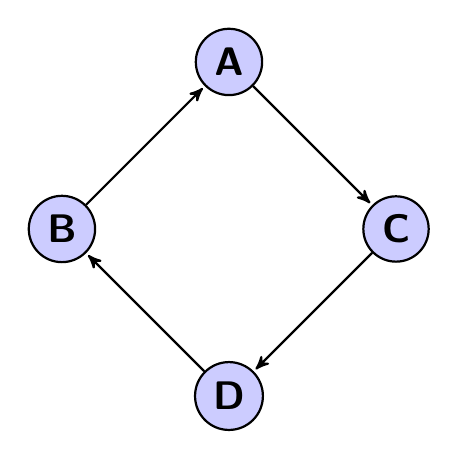
\begin{tikzpicture}[->,>=stealth',shorten >=1pt,auto,node distance=3cm,
  thick,main node/.style={circle,fill=blue!20,draw,font=\sffamily\Large\bfseries}]

  \node[main node] (1) {A};
  \node[main node] (2) [below left of=1] {B};
  \node[main node] (3) [below right of=2] {D};
  \node[main node] (4) [below right of=1] {C};

  \path[every node/.style={font=\sffamily\small}]
    (1) edge node [left] {} (4)
    (2) edge node [right] {} (1)
    (3) edge node [right] {} (2)
    (4) edge node [left] {} (3);
\end{tikzpicture}
\caption{Markovian Dependent Variables}
\end{figure}



 be random variables, and let $X$ be the
joint assignment of these four variables.



 that take
on the values 1 or 0.



These variables can take on $2^4$ permutations. In general, if we are
interested in the probability of any these permutations we need to
keep track of sixteen separate values.

\begin{align*}
&\Pr(A=0,B=0,C=0,D=0) = P_1 \\
&\Pr(A=1,B=0,C=0,D=0) = P_2 \\
&\Pr(A=0,B=1,C=0,D=0) = P_3 \\
&\vdots \\
&\Pr(A=1,B=1,C=0,D=1) = P_{14} \\
&\Pr(A=1,B=1,C=1,D=0) = P_{15} \\
&\Pr(A=1,B=1,C=1,D=1) = P_{16} 
\end{align*}

However, if these variables are independent, then we only need to know
four values -- the probability of each random variable taking a value.

Independence means that the probability of realizing a permutation of
values factors into the product of each value taking on the
corresponding value.

\begin{equation}
\Pr(A,B,C,D) = \Pr(A)\Pr(B)\Pr(C)\Pr(D)
\end{equation}

\section*{Representing Dependence}

We can represent the dependence and independence relations between random
variables in a graph. If the four variables are independent, then we draw
the variables as nodes with no edges between them.


\begin{figure}[!ht]
\centering
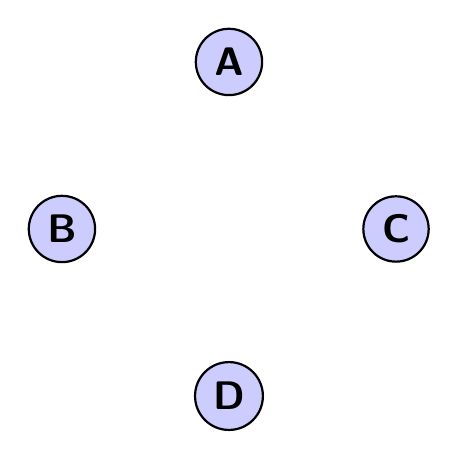
\begin{tikzpicture}[->,>=stealth',shorten >=1pt,auto,node distance=3cm,
  thick,main node/.style={circle,fill=blue!20,draw,font=\sffamily\Large\bfseries}]

  \node[main node] (1) {A};
  \node[main node] (2) [below left of=1] {B};
  \node[main node] (3) [below right of=2] {D};
  \node[main node] (4) [below right of=1] {C};


\end{tikzpicture}
\caption{Completely Independent Variables}
\end{figure}

On the other hand, if each variable is dependent on all the others,
then the graph is completely connected. 

\begin{figure}
\centering
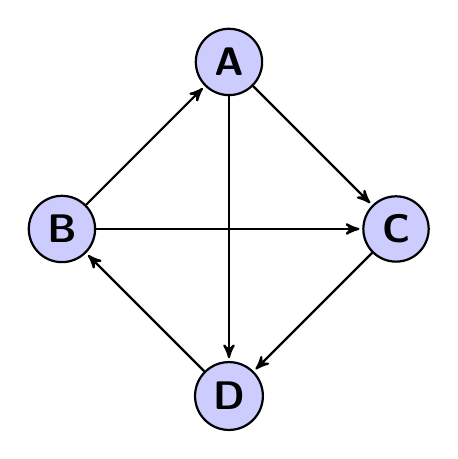
\begin{tikzpicture}[->,>=stealth',shorten >=1pt,auto,node distance=3cm,
  thick,main node/.style={circle,fill=blue!20,draw,font=\sffamily\Large\bfseries}]

  \node[main node] (1) {A};
  \node[main node] (2) [below left of=1] {B};
  \node[main node] (3) [below right of=2] {D};
  \node[main node] (4) [below right of=1] {C};

  \path[every node/.style={font=\sffamily\small}]
    (1) edge node [left] {} (4)
        edge node [left] {} (3)
    (2) edge node [right] {} (1)
        edge node {} (4)
    (3) edge node [right] {} (2)
    (4) edge node [left] {} (3);
\end{tikzpicture}
\caption{Completely Dependent Variables}
\end{figure}

Now, let's consider an intermediate graph. In this graph, conditional
on its neighbors, a random value is independent of all other values. 

\begin{figure}
\centering
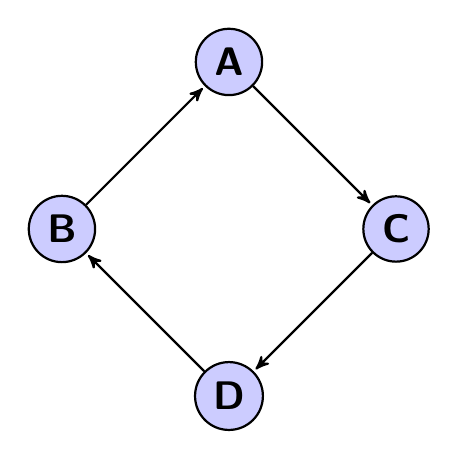
\begin{tikzpicture}[->,>=stealth',shorten >=1pt,auto,node distance=3cm,
  thick,main node/.style={circle,fill=blue!20,draw,font=\sffamily\Large\bfseries}]

  \node[main node] (1) {A};
  \node[main node] (2) [below left of=1] {B};
  \node[main node] (3) [below right of=2] {D};
  \node[main node] (4) [below right of=1] {C};

  \path[every node/.style={font=\sffamily\small}]
    (1) edge node [left] {} (4)
    (2) edge node [right] {} (1)
    (3) edge node [right] {} (2)
    (4) edge node [left] {} (3);
\end{tikzpicture}
\caption{Markovian Dependent Variables}
\end{figure}

Unlike the first case. $A\not\independent D$ and $B\not\independent
C$, but $(A\independent D) \mid (B,C)$, and $(B\independent C) \mid
(A,D)$.

\end{document}